% Options for packages loaded elsewhere
\PassOptionsToPackage{unicode}{hyperref}
\PassOptionsToPackage{hyphens}{url}
\PassOptionsToPackage{dvipsnames,svgnames,x11names}{xcolor}
%
\documentclass[
  letterpaper,
  DIV=11,
  numbers=noendperiod]{scrartcl}

\usepackage{amsmath,amssymb}
\usepackage{iftex}
\ifPDFTeX
  \usepackage[T1]{fontenc}
  \usepackage[utf8]{inputenc}
  \usepackage{textcomp} % provide euro and other symbols
\else % if luatex or xetex
  \usepackage{unicode-math}
  \defaultfontfeatures{Scale=MatchLowercase}
  \defaultfontfeatures[\rmfamily]{Ligatures=TeX,Scale=1}
\fi
\usepackage{lmodern}
\ifPDFTeX\else  
    % xetex/luatex font selection
\fi
% Use upquote if available, for straight quotes in verbatim environments
\IfFileExists{upquote.sty}{\usepackage{upquote}}{}
\IfFileExists{microtype.sty}{% use microtype if available
  \usepackage[]{microtype}
  \UseMicrotypeSet[protrusion]{basicmath} % disable protrusion for tt fonts
}{}
\makeatletter
\@ifundefined{KOMAClassName}{% if non-KOMA class
  \IfFileExists{parskip.sty}{%
    \usepackage{parskip}
  }{% else
    \setlength{\parindent}{0pt}
    \setlength{\parskip}{6pt plus 2pt minus 1pt}}
}{% if KOMA class
  \KOMAoptions{parskip=half}}
\makeatother
\usepackage{xcolor}
\setlength{\emergencystretch}{3em} % prevent overfull lines
\setcounter{secnumdepth}{-\maxdimen} % remove section numbering
% Make \paragraph and \subparagraph free-standing
\ifx\paragraph\undefined\else
  \let\oldparagraph\paragraph
  \renewcommand{\paragraph}[1]{\oldparagraph{#1}\mbox{}}
\fi
\ifx\subparagraph\undefined\else
  \let\oldsubparagraph\subparagraph
  \renewcommand{\subparagraph}[1]{\oldsubparagraph{#1}\mbox{}}
\fi

\usepackage{color}
\usepackage{fancyvrb}
\newcommand{\VerbBar}{|}
\newcommand{\VERB}{\Verb[commandchars=\\\{\}]}
\DefineVerbatimEnvironment{Highlighting}{Verbatim}{commandchars=\\\{\}}
% Add ',fontsize=\small' for more characters per line
\usepackage{framed}
\definecolor{shadecolor}{RGB}{241,243,245}
\newenvironment{Shaded}{\begin{snugshade}}{\end{snugshade}}
\newcommand{\AlertTok}[1]{\textcolor[rgb]{0.68,0.00,0.00}{#1}}
\newcommand{\AnnotationTok}[1]{\textcolor[rgb]{0.37,0.37,0.37}{#1}}
\newcommand{\AttributeTok}[1]{\textcolor[rgb]{0.40,0.45,0.13}{#1}}
\newcommand{\BaseNTok}[1]{\textcolor[rgb]{0.68,0.00,0.00}{#1}}
\newcommand{\BuiltInTok}[1]{\textcolor[rgb]{0.00,0.23,0.31}{#1}}
\newcommand{\CharTok}[1]{\textcolor[rgb]{0.13,0.47,0.30}{#1}}
\newcommand{\CommentTok}[1]{\textcolor[rgb]{0.37,0.37,0.37}{#1}}
\newcommand{\CommentVarTok}[1]{\textcolor[rgb]{0.37,0.37,0.37}{\textit{#1}}}
\newcommand{\ConstantTok}[1]{\textcolor[rgb]{0.56,0.35,0.01}{#1}}
\newcommand{\ControlFlowTok}[1]{\textcolor[rgb]{0.00,0.23,0.31}{#1}}
\newcommand{\DataTypeTok}[1]{\textcolor[rgb]{0.68,0.00,0.00}{#1}}
\newcommand{\DecValTok}[1]{\textcolor[rgb]{0.68,0.00,0.00}{#1}}
\newcommand{\DocumentationTok}[1]{\textcolor[rgb]{0.37,0.37,0.37}{\textit{#1}}}
\newcommand{\ErrorTok}[1]{\textcolor[rgb]{0.68,0.00,0.00}{#1}}
\newcommand{\ExtensionTok}[1]{\textcolor[rgb]{0.00,0.23,0.31}{#1}}
\newcommand{\FloatTok}[1]{\textcolor[rgb]{0.68,0.00,0.00}{#1}}
\newcommand{\FunctionTok}[1]{\textcolor[rgb]{0.28,0.35,0.67}{#1}}
\newcommand{\ImportTok}[1]{\textcolor[rgb]{0.00,0.46,0.62}{#1}}
\newcommand{\InformationTok}[1]{\textcolor[rgb]{0.37,0.37,0.37}{#1}}
\newcommand{\KeywordTok}[1]{\textcolor[rgb]{0.00,0.23,0.31}{#1}}
\newcommand{\NormalTok}[1]{\textcolor[rgb]{0.00,0.23,0.31}{#1}}
\newcommand{\OperatorTok}[1]{\textcolor[rgb]{0.37,0.37,0.37}{#1}}
\newcommand{\OtherTok}[1]{\textcolor[rgb]{0.00,0.23,0.31}{#1}}
\newcommand{\PreprocessorTok}[1]{\textcolor[rgb]{0.68,0.00,0.00}{#1}}
\newcommand{\RegionMarkerTok}[1]{\textcolor[rgb]{0.00,0.23,0.31}{#1}}
\newcommand{\SpecialCharTok}[1]{\textcolor[rgb]{0.37,0.37,0.37}{#1}}
\newcommand{\SpecialStringTok}[1]{\textcolor[rgb]{0.13,0.47,0.30}{#1}}
\newcommand{\StringTok}[1]{\textcolor[rgb]{0.13,0.47,0.30}{#1}}
\newcommand{\VariableTok}[1]{\textcolor[rgb]{0.07,0.07,0.07}{#1}}
\newcommand{\VerbatimStringTok}[1]{\textcolor[rgb]{0.13,0.47,0.30}{#1}}
\newcommand{\WarningTok}[1]{\textcolor[rgb]{0.37,0.37,0.37}{\textit{#1}}}

\providecommand{\tightlist}{%
  \setlength{\itemsep}{0pt}\setlength{\parskip}{0pt}}\usepackage{longtable,booktabs,array}
\usepackage{calc} % for calculating minipage widths
% Correct order of tables after \paragraph or \subparagraph
\usepackage{etoolbox}
\makeatletter
\patchcmd\longtable{\par}{\if@noskipsec\mbox{}\fi\par}{}{}
\makeatother
% Allow footnotes in longtable head/foot
\IfFileExists{footnotehyper.sty}{\usepackage{footnotehyper}}{\usepackage{footnote}}
\makesavenoteenv{longtable}
\usepackage{graphicx}
\makeatletter
\def\maxwidth{\ifdim\Gin@nat@width>\linewidth\linewidth\else\Gin@nat@width\fi}
\def\maxheight{\ifdim\Gin@nat@height>\textheight\textheight\else\Gin@nat@height\fi}
\makeatother
% Scale images if necessary, so that they will not overflow the page
% margins by default, and it is still possible to overwrite the defaults
% using explicit options in \includegraphics[width, height, ...]{}
\setkeys{Gin}{width=\maxwidth,height=\maxheight,keepaspectratio}
% Set default figure placement to htbp
\makeatletter
\def\fps@figure{htbp}
\makeatother

\KOMAoption{captions}{tableheading}
\makeatletter
\makeatother
\makeatletter
\makeatother
\makeatletter
\@ifpackageloaded{caption}{}{\usepackage{caption}}
\AtBeginDocument{%
\ifdefined\contentsname
  \renewcommand*\contentsname{Table of contents}
\else
  \newcommand\contentsname{Table of contents}
\fi
\ifdefined\listfigurename
  \renewcommand*\listfigurename{List of Figures}
\else
  \newcommand\listfigurename{List of Figures}
\fi
\ifdefined\listtablename
  \renewcommand*\listtablename{List of Tables}
\else
  \newcommand\listtablename{List of Tables}
\fi
\ifdefined\figurename
  \renewcommand*\figurename{Figure}
\else
  \newcommand\figurename{Figure}
\fi
\ifdefined\tablename
  \renewcommand*\tablename{Table}
\else
  \newcommand\tablename{Table}
\fi
}
\@ifpackageloaded{float}{}{\usepackage{float}}
\floatstyle{ruled}
\@ifundefined{c@chapter}{\newfloat{codelisting}{h}{lop}}{\newfloat{codelisting}{h}{lop}[chapter]}
\floatname{codelisting}{Listing}
\newcommand*\listoflistings{\listof{codelisting}{List of Listings}}
\makeatother
\makeatletter
\@ifpackageloaded{caption}{}{\usepackage{caption}}
\@ifpackageloaded{subcaption}{}{\usepackage{subcaption}}
\makeatother
\makeatletter
\@ifpackageloaded{tcolorbox}{}{\usepackage[skins,breakable]{tcolorbox}}
\makeatother
\makeatletter
\@ifundefined{shadecolor}{\definecolor{shadecolor}{rgb}{.97, .97, .97}}
\makeatother
\makeatletter
\makeatother
\makeatletter
\makeatother
\ifLuaTeX
  \usepackage{selnolig}  % disable illegal ligatures
\fi
\IfFileExists{bookmark.sty}{\usepackage{bookmark}}{\usepackage{hyperref}}
\IfFileExists{xurl.sty}{\usepackage{xurl}}{} % add URL line breaks if available
\urlstyle{same} % disable monospaced font for URLs
\hypersetup{
  pdftitle={Glyph-Maps-Test},
  pdfauthor={Maliny Po},
  colorlinks=true,
  linkcolor={blue},
  filecolor={Maroon},
  citecolor={Blue},
  urlcolor={Blue},
  pdfcreator={LaTeX via pandoc}}

\title{Glyph-Maps-Test}
\author{Maliny Po}
\date{}

\begin{document}
\maketitle
\ifdefined\Shaded\renewenvironment{Shaded}{\begin{tcolorbox}[boxrule=0pt, frame hidden, enhanced, borderline west={3pt}{0pt}{shadecolor}, breakable, interior hidden, sharp corners]}{\end{tcolorbox}}\fi

\hypertarget{glyph-map-for-cubble-package}{%
\section{\texorpdfstring{Glyph map for
\texttt{cubble\ package}}{Glyph map for cubble package}}\label{glyph-map-for-cubble-package}}

A descriptive title of the project that you want to work on

\hypertarget{about-me}{%
\section{About Me}\label{about-me}}

Description of your programming experience, attained education,
university and study programme that you're currently studying, etc. (a
short CV would be ideal) Link to a portfolio of projects that you have
worked on (e.g.~a GitHub profile or a personal website) Your knowledge
of Rust, since most projects will probably require at least some Rust
knowledge Your existing open-source contribution experience. If you have
already contributed to some open-source repositories, make sure to
include a link to these contributions in your proposal! Your preferred
time zone (for communicating with the mentor(s)) Contact information

\hypertarget{tests}{%
\section{Tests}\label{tests}}

\hypertarget{easy-run-the-glyph-map-examples}{%
\subsubsection{Easy: Run the glyph map
examples}\label{easy-run-the-glyph-map-examples}}

\begin{Shaded}
\begin{Highlighting}[]
\CommentTok{\# Run the glyph map example}
\NormalTok{print\_p }\OtherTok{\textless{}{-}}\NormalTok{ GGally}\SpecialCharTok{::}\NormalTok{print\_if\_interactive}
\end{Highlighting}
\end{Shaded}

\begin{verbatim}
Registered S3 method overwritten by 'GGally':
  method from   
  +.gg   ggplot2
\end{verbatim}

\begin{Shaded}
\begin{Highlighting}[]
\CommentTok{\# basic glyph map with reference line and box{-}{-}{-}{-}{-}{-}{-}{-}{-}{-}{-}{-}{-}{-}{-}}
\NormalTok{p }\OtherTok{\textless{}{-}} \FunctionTok{ggplot}\NormalTok{(}\AttributeTok{data =}\NormalTok{ GGally}\SpecialCharTok{::}\NormalTok{nasa,}
       \FunctionTok{aes}\NormalTok{(}\AttributeTok{x\_major =}\NormalTok{ long, }\AttributeTok{x\_minor =}\NormalTok{ day,}
           \AttributeTok{y\_major =}\NormalTok{ lat, }\AttributeTok{y\_minor =}\NormalTok{ surftemp)) }\SpecialCharTok{+}
  \FunctionTok{geom\_glyph\_box}\NormalTok{() }\SpecialCharTok{+}
  \FunctionTok{geom\_glyph\_line}\NormalTok{() }\SpecialCharTok{+}
  \FunctionTok{geom\_glyph}\NormalTok{() }\SpecialCharTok{+}
  \FunctionTok{theme\_bw}\NormalTok{()}
\FunctionTok{print\_p}\NormalTok{(p)}
\end{Highlighting}
\end{Shaded}

\hypertarget{medium-create-an-example-to-be-used-as-a-glyph-on-a-map}{%
\subsubsection{Medium: Create an example to be used as a glyph on a
map}\label{medium-create-an-example-to-be-used-as-a-glyph-on-a-map}}

\begin{Shaded}
\begin{Highlighting}[]
\CommentTok{\# Define bounds for Central America}
\NormalTok{xlim }\OtherTok{\textless{}{-}} \FunctionTok{c}\NormalTok{(}\SpecialCharTok{{-}}\DecValTok{112}\NormalTok{, }\SpecialCharTok{{-}}\DecValTok{58}\NormalTok{) }\CommentTok{\# Longitude bounds for Central America}
\NormalTok{ylim }\OtherTok{\textless{}{-}} \FunctionTok{c}\NormalTok{(}\SpecialCharTok{{-}}\FloatTok{19.5}\NormalTok{, }\DecValTok{35}\NormalTok{) }\CommentTok{\# Latitude bounds for Central America}


\CommentTok{\# Subset for observations in 2000}
\NormalTok{climate\_data }\OtherTok{\textless{}{-}}\NormalTok{ GGally}\SpecialCharTok{::}\NormalTok{nasa }\SpecialCharTok{|\textgreater{}}
  \FunctionTok{filter}\NormalTok{(lubridate}\SpecialCharTok{::}\FunctionTok{year}\NormalTok{(date) }\SpecialCharTok{==} \DecValTok{2000}\NormalTok{)}
\end{Highlighting}
\end{Shaded}

\begin{Shaded}
\begin{Highlighting}[]
\CommentTok{\# Base map with geom\_roster displaying the Ozone value}
\NormalTok{base\_plot }\OtherTok{\textless{}{-}} \FunctionTok{ggplot}\NormalTok{(climate\_data, }\FunctionTok{aes}\NormalTok{(}\AttributeTok{x =}\NormalTok{ long, }\AttributeTok{y =}\NormalTok{ lat)) }\SpecialCharTok{+}
  \FunctionTok{geom\_raster}\NormalTok{(}\FunctionTok{aes}\NormalTok{(}\AttributeTok{fill =}\NormalTok{ ozone)) }\SpecialCharTok{+} \CommentTok{\# Adjust \textquotesingle{}size\textquotesingle{} as needed}
  \FunctionTok{borders}\NormalTok{(}\StringTok{"world"}\NormalTok{, }\AttributeTok{fill=}\StringTok{"grey7"}\NormalTok{, }\AttributeTok{alpha =} \FloatTok{0.3}\NormalTok{) }\SpecialCharTok{+}
  \FunctionTok{scale\_fill\_gradientn}\NormalTok{(}\AttributeTok{colors =} \FunctionTok{c}\NormalTok{(}\StringTok{"\#0000FFFF"}\NormalTok{,}\StringTok{"\#FFFFFFFF"}\NormalTok{,}\StringTok{"\#FF0000FF"}\NormalTok{)) }\SpecialCharTok{+}
  \FunctionTok{labs}\NormalTok{(}\AttributeTok{title =} \StringTok{"Spatial Dynamics of Ozone and Surface Temperature Across }
\StringTok{South America, 2000"}\NormalTok{,}
       \AttributeTok{subtitle =} \StringTok{"Ozone Levels Visualized by Intensity on a Geom{-}Raster Overlay"}\NormalTok{,}
       \AttributeTok{x =} \StringTok{"Longitude"}\NormalTok{, }\AttributeTok{y =} \StringTok{"Latitude"}\NormalTok{,}
       \AttributeTok{color =} \StringTok{"Surface Temp"}\NormalTok{) }\SpecialCharTok{+} \CommentTok{\# Add a simple world map as background}
  \FunctionTok{coord\_fixed}\NormalTok{(}\AttributeTok{xlim =}\NormalTok{ xlim, }\AttributeTok{ylim =}\NormalTok{ ylim) }
\end{Highlighting}
\end{Shaded}

\begin{Shaded}
\begin{Highlighting}[]
\CommentTok{\# Set up}

\DocumentationTok{\#\# Function to create a time series plot glyph for each grid}
\NormalTok{plot\_glyph }\OtherTok{\textless{}{-}} \ControlFlowTok{function}\NormalTok{(data) \{}
\NormalTok{  data }\SpecialCharTok{|\textgreater{}}
    \FunctionTok{ggplot}\NormalTok{(}\FunctionTok{aes}\NormalTok{(}\AttributeTok{x =}\NormalTok{ date, }\AttributeTok{y =}\NormalTok{ surftemp)) }\SpecialCharTok{+}
    \FunctionTok{geom\_line}\NormalTok{(}\AttributeTok{group =} \DecValTok{1}\NormalTok{, }\AttributeTok{color =} \StringTok{"black"}\NormalTok{) }\SpecialCharTok{+}
    \FunctionTok{theme\_void}\NormalTok{() }\SpecialCharTok{+}
    \FunctionTok{theme}\NormalTok{(}\AttributeTok{panel.border =} \FunctionTok{element\_blank}\NormalTok{())}
\NormalTok{\}}

\DocumentationTok{\#\# Find unique combination of longitude and latitude}
\NormalTok{unique\_grid }\OtherTok{\textless{}{-}} \FunctionTok{unique}\NormalTok{(climate\_data}\SpecialCharTok{$}\NormalTok{id) }

\DocumentationTok{\#\# Value for horizontal, vertical location of raster}
\NormalTok{x\_size }\OtherTok{\textless{}{-}} \DecValTok{1} 
\NormalTok{y\_size }\OtherTok{\textless{}{-}} \DecValTok{1}
\end{Highlighting}
\end{Shaded}

\begin{Shaded}
\begin{Highlighting}[]
\CommentTok{\# Add Glyph }
\ControlFlowTok{for}\NormalTok{ (i }\ControlFlowTok{in}\NormalTok{ unique\_grid) \{}
  
\NormalTok{  data }\OtherTok{\textless{}{-}}\NormalTok{ climate\_data }\SpecialCharTok{|\textgreater{}}
    \FunctionTok{filter}\NormalTok{(id }\SpecialCharTok{==}\NormalTok{ i)}
  
\NormalTok{  lat\_val }\OtherTok{\textless{}{-}}\NormalTok{  data}\SpecialCharTok{$}\NormalTok{lat[}\DecValTok{1}\NormalTok{] }\CommentTok{\# Latitude at grid i}
\NormalTok{  long\_val }\OtherTok{\textless{}{-}}\NormalTok{ data}\SpecialCharTok{$}\NormalTok{long[}\DecValTok{1}\NormalTok{] }\CommentTok{\# Longitude at grid i}
  
  \CommentTok{\# Create the glyph using the custom \textasciigrave{}plot\_glyph\textasciigrave{} function}
\NormalTok{  p }\OtherTok{\textless{}{-}} \FunctionTok{plot\_glyph}\NormalTok{(data)}
  
  \CommentTok{\# Add the glyph as an annotation}
\NormalTok{  base\_plot }\OtherTok{\textless{}{-}}\NormalTok{ base\_plot }\SpecialCharTok{+} 
    \FunctionTok{annotation\_custom}\NormalTok{(}\FunctionTok{ggplotGrob}\NormalTok{(p), }
                      \AttributeTok{xmin =}\NormalTok{ long\_val }\SpecialCharTok{{-}}\NormalTok{ x\_size, }\AttributeTok{xmax =}\NormalTok{ long\_val }\SpecialCharTok{+}\NormalTok{ x\_size,}
                      \AttributeTok{ymin =}\NormalTok{ lat\_val }\SpecialCharTok{{-}}\NormalTok{ y\_size, }\AttributeTok{ymax =}\NormalTok{ lat\_val }\SpecialCharTok{+}\NormalTok{ y\_size)}
\NormalTok{\}}

\CommentTok{\# Print the Glyph Map}
\FunctionTok{print}\NormalTok{(base\_plot) }
\end{Highlighting}
\end{Shaded}

\begin{figure}[H]

{\centering 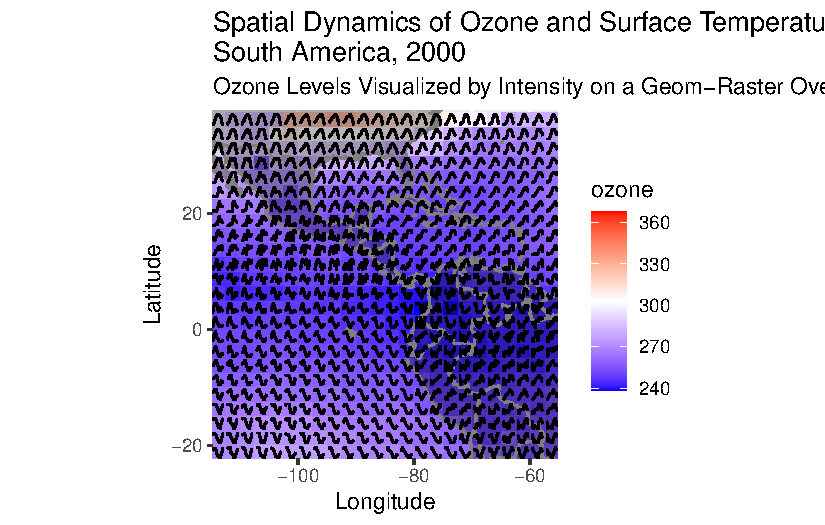
\includegraphics{Test_files/figure-pdf/unnamed-chunk-6-1.pdf}

}

\end{figure}

To illustrate the dynamic interplay between ozone levels and surface
temperature across South America in 2000, I constructed a glyph map with
a two-fold visual approach. First, I established a base map utilizing
geom\_raster to display ozone values, overlaid with the continent's
silhouette for geographical context. This raster layer employs a
gradient color scheme, transitioning from blue to red, to represent the
varying intensities of ozone concentration.

The second layer of visualization introduces the glyph element: a series
of line graphs representing the time series of surface temperatures for
each unique grid location. I crafted these glyphs with a custom
function, plot\_glyph, designed to generate a line plot for the given
data slice.

For each grid point, identified by its unique id, I extracted the
corresponding latitude and longitude values and deployed the plot\_glyph
function to produce a miniaturized time series plot. This glyph
encapsulates the temporal pattern of surface temperatures throughout the
year 2000.

I then meticulously positioned each glyph onto the base map using
annotation\_custom, aligning them with their geographic counterparts and
fine-tuning their spatial footprint through xmin, xmax, ymin, and ymax
parameters. The resulting visualization is a composite map that fuses
the static backdrop of ozone distribution with the dynamic narrative of
temperature fluctuations, offering a nuanced perspective on
environmental patterns over space and time.

\hypertarget{hard-small-change-to-geom_glyph-in-the-cubble-package-and-create-a-pull-request}{%
\subsubsection{\texorpdfstring{HARD: Small change to
\texttt{geom\_glyph} in the cubble package and create a pull
request}{HARD: Small change to geom\_glyph in the cubble package and create a pull request}}\label{hard-small-change-to-geom_glyph-in-the-cubble-package-and-create-a-pull-request}}

My pull request can be found at: \href{}{link}.



\end{document}
